\chapter{Existing solutions}
\label{cha:solutions}

In the previous chapter we discussed some of the philosophy of distributive ethics, but it is also important to consider the way those ideas can be made quantitatively precise.

In this chapter we consider some of ways that moral ideas about distribution can be mathemetised.
We highlight some of the most famous and relevent formulations, primarily because our development extends from them, and also ultimately contrasts against them.

We consider the following formulations:
\begin{itemize}
\item VCG,
\item Locational Marginal Pricing,
\item nash bargaining with and without endogenous disagreement point,
\item and cooperative game theory concepts including the Core and Shapley Value.
\end{itemize}

We introduce, consider and discuss the qualities of each of these in turn, before we attempt a new synthesis in the next chapter \ref{}.
let us begin with the VCG mechanism.

\section{VCG}

In section \ref{sec:reference_points} we briefly presented the idea that people might be rewarded in proportion to their contribution to social welfare, above their absense individually.
While this idea may be simple, its mathematization has some suprising features.
The most direct mathemetisation of this idea, is the Vickery-Clark-Groves (VCG) mechanism with Clark pivot.

The VCG mechanism (with Clark pivot) is an allocation process where each player is payed money (or `transferable utility') equal to the impact that their presense has apon others (ie. their externality) in the decision process which selecting an outcome that maximises the sum of utility.
Let us explain with some mathematics:

\subsection{The minimal VCG process - with Clark pivot}
If we frame the VCG process as a bidding process of $n$ agents over a possible set of outcomes $X$.
We assume that every agent $i$ has a valuation (or utility) $v_i$ for any outcome in $X$:
$$ v_i~:~X\rightarrow \mathbb{R}_{\ge 0} $$
The VCG bidding process asks every agent $i$ for their valuations and calculates the outcome that maximises the sum of the reported valuations:
$$ x^*(v) = \argmax_{x\in X}\sum_{i=1}^{n}v_i(x) $$
This outcome is implemented and the bidding process pays each agent $i$ the utility value $p_i$ (which may be positive or negative):
\begin{equation}\label{eq:VCG_payment_rule} p_i(v)=\sum_{j\ne i}v_j(x^*(v)) - \max_{x'\in X}\sum_{j\ne i}v_j(x') \end{equation}
And this value $p_i$ is the value that the player's presence adds to the utility of others minus the sum of their utility which would have been obtained in the player's absense - ie. the player's externality.

\subsection{Discussion about VCG}
The VCG mechanism with Clark pivot might be seen as an straightforward way of allocating ethical payments; if a player's presence adds to the utility of others then they are postiviely compensated, and if a player's influence detracts from the utility of others then they are negatively compensated.

And since the set of possible outcomes $X$ are undefined it is possible to consider the application of the VCG mechanism in a variety of contexts.	
For instance, VCG has been considered as a mechanism for allocating physical and monetary outcomes in various contexts within electricity networks, such as in auctions for bulk electricity generation, buying and selling energy storage products, and in procuring ancillary services \cite{FABRA200272, SESSA2017189, 8264596, 7512339}.

However VCG has some particular advantages and disadvantages.
The first and most notable property is that VCG mechanisms are \textit{truthfull} or \textit{incentive compatable}, in that no player can possibly gain from misreporting their valuations
in the event that the utility of the agents is \textit{quasilinear} \cite{roberts1979characterization, Lavi2008}, ie. that their net utility is equal to their valuation of the outcome plus any transfers they recieve, and their utility $u_i$ has form:
$$ u_i = p_i(v)+v_i $$
And thus if incentive compatability induces the players not to bid strategically, then it reduces a potential overhead of their participation in the system, and also potentially eliminates a source of instability in the resulting system.

Another interesting property is sometimes called \textit{individual rationality}, in that no agent (assuming quasilinear utility) will ever be left with a net negative utility. Particularly if the utility of zero is regarded as the utility of non-participation, then invidually rational means that everybody is left being better-off by participating than they would be otherwise. Hence individual rationality is possible a minimal component of ethical euvolentary negotiation (see chapter \ref{}).

It is also worth noting that VCG mechanisms are also \textit{efficient} in the sense that the process actualises the utilitarian socially optimal solution $x^*(v) \in X$.

However more negative features of VCG exist, one primary drawback of this mechanism is that it is not \textit{budget balanced}, in that it is possible for the amount of utility that is transferred between the players might not sum to zero; and hence an implementation of VCG might require regular budget injection to maintain and/or sap money from between the participants.

Although VCG is incentive compatable for individual strategisers it is potentially vulnerabile to strategising coalitions, additionally its implementation may involve imposing a lack of privacy for participants, and also (depending on context) may also have higher computational complexity than other mechanisms.\cite{ShohamLeytonBrown09}

Some of these disadvantages (and others) have made VCG seldom implemented in practice, and in electricity networks.\cite{Rothkopf07, Ausubel2006}

As VCG has positive and negative features, it is possible to ask if there are similar mechanisms which avoid some of the negative features.
But it is unfortunate, that some of these properties (incentive compatable, individually rational, budget balanced, and efficiency) are known to be impossible to combine in the general case (where there are a plurality of outcomes and the valuations are unrestricted), and these impossibility theorems are a component feature in the study of \textit{Mechanism Design}.%(find a good source, of, myerson satterthwaite theorem)

\subsection{Mechanism Design, is there a better VCG?}

The VCG mechanism is a cornerstone component in the field of Mechanism Design, and there exist many good sources giving extended discussions on the field.\cite{37377}
But generally, Mechanism Design analyses systems which select social outcome/s based apon the result of strategic interactions of multiple parties with divergent interests.% and where each party has actual preferences over the possible outcomes, and also reported preferences over the outcomes.

One of the features of Mechanism design that the VCG mechanism illustrates, is the potential for considering and apprehending the way in which a system is likely to behave between rational individual strategising agents.
This possibility extends beyond VCG, as it has been discovered that any system which is implemented between strategising agents can be altered such as to make it incentive compatable for them; and this is called the revelation principle.\cite{RePEc:ecm:emetrp:v:41:y:1973:i:4:p:587-601} \cite[Chapter~2.3]{37377}
The revelation principle has various formulations, but generally, for any system there will nash-equilibria in the interaction between the agents, and consequently an incentive compatable mechanism can be constructed by asking the agents for their true valuations and then implimenting the corresponding nash equilibria directly.
Unfortunately, it is sometimes the case that the nash-equilibria between strategising agents may not coincide with what is socially optimal for them; and the general difficulty of designing systems where the socially optimal outcome is always created as nash equilibrium is rendered in some of the famous impossibility theorems in Mechanism Design. %And so, there are a series of strong impossibility proofs in mechanism design.

Some historic impossibility proofs in mechanism design concern voting and social choice, and notably include Arrow's impossibility theorem, and the Gibbard-Satterthwaite theorem.
But the difficulty does not nessisarily receed even if monetary compensations between parties are included into consideration. such as per the Myerson-Satterthwaite theorem.
Another impossibility theorem was also proven by Green and Laffont \cite{29088} to the effect of proving that there is no easy alternative to VCG; ie. a mechanism which is incentive compatabile, has unrestricted player preferences, has individual rationality, and implements a socially optimal outcome.

In the evolving field of Mechanism Design there are several avenues of averting some of the impossibilities.

%\subsection{Navigating around impossibilities of Mechanism Design to a better VCG}

One of the main problems in applying VCG to electricity networks is the fact that it is not budget-balanced, and this raises a question of where the budget surplus/defecit should be channeled to/from.
Particularly if the money should be directed back to the participants in the electricity network, then it would destroy the incentive compatability that was part of the scheme in the first place.
And this is a direct consequence of the impossibility result of Green and Laffont \cite{29088}. By this impossibility result we are constrained to consider mechanisms which are suboptimal in relation to these qualities (budget balance, incentive compatability, individually rational, and efficient).

Subsequently, we could ask if there is any potential mechanisms which are boundedly suboptimal about thoes qualities, and the answer is unfortunately not.
Particularly there are no mechanisms which allow bounded deviations from the efficiency, incentive compatibility and budget-balance at the same time (allowing such mild conditions as quasilinear utilities) \cite{YI201679}.
Thus a search for a better alternative than VCG needs to sacrifice or substitute some of these desirable properties.

And there are several options, such as:
\begin{enumerate}
    \item Discarding the unrestrictedness of the player valuations, and by moving to other Groves mechanisms which allow some redistribution of the surplus
    \item Sacrificing efficiency while keeping budget balance and incentive compatability
    \item Adding baysean priors on the valuations of the players, and reducing incentive compatability to baysean incentive compatability
\end{enumerate}

We briefly discuss these in turn:

\subsubsection{Redistribution in Groves mechanisms}

One potential avenue of averting the impossibility result is to discard the assumption that the player's valuation over outcomes are unrestricted, and recognise that some of the budget surplus/defecit can be redistributed without destroying the incentive compatability property.

To frame this approach, we must make a technical distinction between a Groves mechanism and its particular instance - in the VCG mechanism.
A Groves mechanism is exactly the same as the VCG mechanism except instead of paying players per equation \ref{eq:VCG_payment_rule}, instead it pays them per:
\begin{equation}\label{eq:Groves_payment_equation} p_i(v)=\sum_{j\ne i}v_j(x^*(v)) - C_{-i} \end{equation}
where $C_{-i}$ is some function that is independent of $i$'s reported preferences.
In this context it is notable that the VCG mechanism is a special case of a Groves mechanism where $C_{-i}= \max_{x'\in X}\sum_{j\ne i}v_j(x')$. \cite{10.2307/1914085}
Groves mechanisms are a class of mechanisms which include VCG, and are categorically incentive compatable. 

The challenge therefore is to derive optimal functions $C_{-i}$ which minimise the budget surplus/defecit while maintaining individual rationality in the context of restricted player valuations.
And to this challenge has been significant discussion about deriving these $C_{-i}$ functions, also known as `VCG redistribution' rules.

One of the first people to propose such a rule was Ruggiero Cavallo \cite{Cavallo:2006:ODM:1160633.1160790}.% who showed that such a redistribution rule exists with with a performance exceeding VCG.
Who showed that much of the VCG surplus can be redistributed in a process of allocating a single physical object exclusively to one party (called `All-Or-Nothing' games), where it can be assumed that any party has a utility of zero if the do not recieve the physical object.
This redistribution was possible primarily because there exists a simple constraint on player valuations - ie. not reciving the object has utility of zero.

Similarly in other situations where there are restrictions on the players valuation over the outcomes, there is the potential for deriving VCG redistribution rules.

However there are some difficulties with this approach, particularly it is known that even with VCG redistribution rules there will almost always be some remaining budget surplus, and even then the process of deriving optimal redistribution rules can be a difficult and complex task --- even to the point where neural networks have been employed to construct such functions \cite{DBLP:conf/atal/ManishaJG18}.

\subsubsection{Sacrificing efficiency}

Anoher avenue in dealing with the problem is to sacrifice efficiency of outcome selection.
One of the simplest such scheme is given by Boi Faltings \cite{10.1007/978-3-642-25510-6_14}
Who proceeds about the process of designing a non-pareto optimal VCG mechanism by splitting the population into two groups, where the VCG outcome from the first group is selected irrespective of the preferencs in the second group.
and where the second group recieves the budget surplus from the VCG mechanism applied to the first group.
This rather genius mechanism is the subject of a patent in the US (CITE), and constitutes a budget balanced VCG-type mechanism.
which can be made a little bit more baysean regular by randomy selecting the `sink', and splitting the budget surplus between the parties evenly without knowledge of who will be selected.\cite{10.1007/978-3-642-25510-6_14}

particularly this method selecting a non-pareto optimal outcome has been the subject of investigation, and the process is proven to nessisarily need a sink.
and that there are different ways to select an appropriate sink randomly \cite{NATH2019673}.



\subsubsection{switching to Baysean incentive compatability}

is the source of the d'AVGA mechanism which allocates redistribution of the surplus bassed on baysean priors on player preferences.
The addition of baysean priors also has links to bargaining, particularly with the work of Meyerson, and his bargaining games.
Which in turn have been extened (by himself) to coalitional games, and also through some of his work to Harsanyi games. (CITE)
Particularly through the introduction of baysean considerations other schemes can redily be made to be incentive compatable.
However there are certain issues with supposing accurately known baysean priors (particularly if they are learnt from past behavior).

 (see section on bargaining)







What is particularly interesting is that various VCG type mechanisms can potentially be scaled up, leading to `effectively' the impossible combination \cite{NATH2019673, 8430852}.

And although incentive compatability is a noble objective in mechanism design, it is still subject to strategic manipulation, particularly in the context of the forming of coalitions.

Coalition strategy proofness, has been proven to be quite generally a difficult concept to design, and in some cases has categorically proven to be impossible \cite{10.2307/2297048} without further elements, such as private information transfer and uncertainty.
Although there has been some effort in designing and analysing the occurance of coalition proof mechanisms, these remain difficult.


In short, the VCG mechanism provides a straightforward ethical schema for distributive payments, and is extensable to electricity systems.
although it is incentive compatable, the primary practical draw-back to such a system is that it is not budget-balanced.
Unfortunately there is no easily implementable system that is like VCG that is incentive compatable and is budget-balanced without forcing participants to trade at a loss.
notwithstanding it is a possible scheme for the trading of electricity and electric resources, and in the following sections \ref{} we will compare the allocations of power/money in randomly generated networks under VCG against other schemes.
Additionally in sections \ref{} we consider the computational difficulty in applying VCG against other schemes.



\subsection{Locational Marginal Pricing, and economic utility}

In Section \ref{sec:reference_points} we briefly considered the notion that moral and euvoluntary trading would result in normative market pricing; and potentially that the morality of a transaction could be framed with respect to the normal market prices.

We saw this in John Locke's short essay Venditio \cite{locke2003locke} where it is argued that a fair price for something is simply its normal market price at its location.\footnote{``... the market price at the place where he sells. Whosoever keeps to that in whatever he sells I think is free from cheat, extortion and oppression, ...''}
John Locke argues this thesis, by arguing that negotiating above market price for a good would be unethical as it would taking advantage of ignorance or special circumstance of the buyer, but that negotiating below market price would only incentivise reselling and allow others to profit at the original seller's loss.
Additionally that selling below market price only to thoes who are needy is certainly a charity and hence cannot be required by justice, but that justice only requires offering no more than the same nominal market price for everybody.

While John Locke's arguments may or may not be convincing, it is usefull to consider the transactions and pricing that would occur under idealised or normative euvoluntary trading.
These prices may be a moral themself, or provide a back-drop for the framing of more moral trading.
In section \ref{sec:solutions_bargaining} we consider mathematical schemas used to describe idealised bargaining between small numbers of participants, but in this section we describe some theory that is used in describing normalised trading en-masse.

%Unfortunately the determination of normalised trading, and normal market price is not nessisarily so easy to distill in practice.
Historic economic thought lend consideration to the idea that market prices can be described by combinations of factors, not limited to, supply and demand functions, market uncertainty, production costings and transport tariffs.
And the combination of these many things are related to the pricing and subsequent trading of the goods.
However, the way in which these factors have been seen to influence (or define) economic value has changed over time.

In the history of economic thought, there was some general idea that the economic value of something (and hence its normal market price) should, in some way, be related to its usefullness in fulfilling human needs - however fickle or not - as things which are utterly useless seldom fetch any price.
%Even so far as to categorising into numbered classes different goods depending on their relation to satisficing needs (eg. \cite[Chapter 1]{mengerprinciples}).
%Such as where different needs (eg. hunger) require first-order goods (eg. bread) to satisfy them, and thoes require second-order goods to provide (eg. flour to make bread), and so on. 
But, above this, there was a difficulty explaining how it was that things which were most usefull to satisfying needs often had little economic value, and things which were more useless were sometimes most economically valuable; is this apparent contradiction is known as the water-diamond paradox, best put by Adam Smith:

%\begin{displayquote}
%The word VALUE, it is to be observed, has two different meanings, and sometimes expresses the utility of some particular object, and sometimes the power of purchasing other goods which the possession of that object conveys. The one may be called `value in use;' the other, `value in exchange.' The things which have the greatest value in use have frequently little or no value in exchange; and, on the contrary, those which have the greatest value in exchange have frequently little or no value in use. Nothing is more useful than water; but it will purchase scarce any thing; scarce any thing can be had in exchange for it. A diamond, on the contrary, has scarce any value in use; but a very great quantity of other goods may frequently be had in exchange for it.\cite{Smith1Gutenberg}
%\end{displayquote}

\begin{displayquote}
The word VALUE, it is to be observed, has two different meanings, ... The things which have the greatest value in use have frequently little or no value in exchange; ... Nothing is more useful than water; but it will purchase scarce any thing; ... A diamond, on the contrary, has scarce any value in use; but a very great quantity of other goods may frequently be had in exchange for it.\cite{Smith1Gutenberg}
\end{displayquote}

To this, there was considered the idea that economic value reflects labor; this `labor theory of value' was held by many authors (including Adam Smith\footnote{The real price of every thing, what every thing really costs to the man who wants to acquire it, is the toil and trouble of acquiring it.\cite{Smith1Gutenberg}}, David Riccardo\footnote{``The value of a commodity, or the quantity of any other commodity for which it will exchange, depends on the relative quantity of labour which is necessary for its production...''\cite[Section 1, Chapter 1]{Riccardo1Gutenberg}}, and many others) but most notably by Karl Marx:

\begin{displayquote}
It suffices to say that if supply and demand equilibrate each other, the market prices of commodities will correspond with their natural prices, that is to say with their values, as determined by the respective quantities of labour required for their production \cite{marx1910value}
\end{displayquote}

And this idea, that the quantity of labor should (in some way) define market prices at market equilibrium, was subject to analysis and verification.
But ultimately the question of how to transform volumes of labor into competitive market prices became a difficult problem known as the `Transformation Problem'.

However the various utilitarians of the 19th century viewed utility no only as a direction of moral efforts, but as a fundamental drive of human behavior\footnote{for instance see Bentham: ``Nature has placed mankind under the governance of two sovereign masters, pain and pleasure.
It is for them alone to point out what we ought to do, as well as to determine what we shall do.''\cite{bentham1823introduction}}, including market behaviors such as price setting; and ultimately, this perspective yeilded a new explanation for economic value.

The utilitarian perspective sought to explain normal market prices in terms of the equilibrium of people's market behavior in maximising their own utility; and this perspective linked economic dynamics with the concept of the margin - or `marginalism'.
Although the concept of marginal dynamics was evidenced in some writings in the earlier half of the 19th century (such as in the works of Jules Dupuit and Hermann Heinrich Gossen), it took to the end of the century for the idea to become more thoroughly developed \cite{RePEc:ucp:jpolec:v:58:y:1950:p:307}.
Although there was much discussion about the relationship between the labor theory of value and marginalism at the end of the 19th century \cite{steedman2003socialism} ultimately marginalism was adopted mainstream in the so-called 'marginal revolution', defining the beginning of neoclassical economics.\cite{Opocher_2017}

The marginalist principles saw that economic values were not just equal to the summation of production costs\footnote{Such as promoted by Riccardo, ``The real and ultimate regulator of the relative value of any two commodities, is the cost of their production, and neither the respective quantities which may be produced, nor the competition amongst the purchasers.''\cite{Riccardo1Gutenberg}} (which then depend on the value of labor), but depends on the cost of production of the most marginal unit produced to meet demand.

The idea of marginalism is best illustrated with a graph, in Figure \ref{fig_demand_supply} we have a hypothetical market for a particular economic good, with many suppliers and many buyers.
In the figure we have the plotted the `Supply curve', identifying how many units of the good could be sustainably supplied to the market if the units sold for a particular price.
And we also have the `Demand curve', identifying how many units of the good would be sold depending on the price which the goods sold at.
If the goods have a set price and the market is functioning ideally, then there is only one sensible outcome: that the goods should be sold in the number (and therefore at the price), that is at the intersection of the supply and demand curves - ie. the marginal price point.
For if there were more goods produced, then thoes excess units would be unsold hence their production would be unprofitable, and if there were less goods produced, then there would be unmet demand which would spur more production.

Different sellers may choose different prices in a market, however if any individual seller tried to deviate from this marginal price in the context of such an ideal market, then it would be a disadvantageous for them.
If a seller tried to set a higher price than the marginal rate then it would result in a failure to sell, or if a seller set a lower price then it would only result in less profit.
In this way, the marginal price point identifies an equilibrium of peoples utility (or profit) maximising efforts.

This kind of marginal analysis is a short sketch of the analysis and treatment in modern microeconomic texts (such as Vohra \cite{vohra_2020}).
And this sort marginalist analysis is also widely regarded to resolve the water-diamond paradox, in that water is cheap because its marginal unit is cheap to produce.

Over time the marginalist synthesis was developed more comprehensively in the presense of many discussions and criticisms.
Particular criticisms attack the academic assertion that market participants are psychologically driven by rational utility maximisation \cite{RePEc:ucp:jpolec:v:58:y:1950:p:307}, and the more pragmatic assertion that markets are approximately ideal and tend towards the stability of equilibrium \cite{nla.cat-vn5739105}.


\begin{figure}[]{}
    \centering
	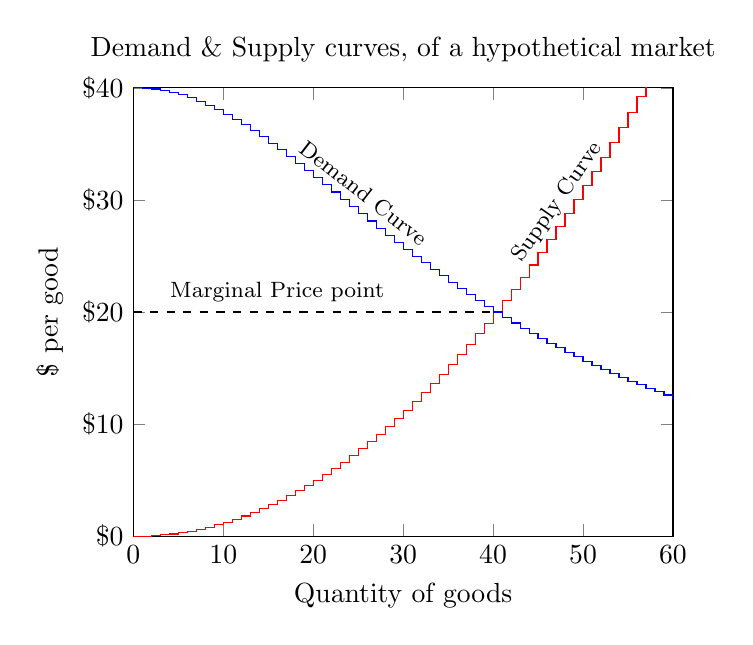
\begin{tikzpicture}
	\begin{axis}[
		title={Demand \& Supply curves, of a hypothetical market},
		xlabel={Quantity of goods},
		ylabel={\$ per good},
		xmin=0, xmax=60,
		ymin=0, ymax=40,
		%xtick={0,0.05,0.1,0.15,0.2,0.25},
		%ytick={30,35,40},
		yticklabel=$\$\pgfmathprintnumber{\tick}$,
		%ymajorgrids=true,
		grid style=dashed,
		xticklabel style={/pgf/number format/fixed},
	]
	\addplot[red] coordinates {
(0,0.0)(1,0.0)(1,0.012500000000000002)(2,0.012500000000000002)(2,0.05000000000000001)(3,0.05000000000000001)(3,0.11249999999999999)(4,0.11249999999999999)(4,0.20000000000000004)(5,0.20000000000000004)(5,0.3125)(6,0.3125)(6,0.44999999999999996)(7,0.44999999999999996)(7,0.6124999999999999)(8,0.6124999999999999)(8,0.8000000000000002)(9,0.8000000000000002)(9,1.0125000000000002)(10,1.0125000000000002)(10,1.25)(11,1.25)(11,1.5125000000000002)(12,1.5125000000000002)(12,1.7999999999999998)(13,1.7999999999999998)(13,2.1125000000000003)(14,2.1125000000000003)(14,2.4499999999999997)(15,2.4499999999999997)(15,2.8125)(16,2.8125)(16,3.2000000000000006)(17,3.2000000000000006)(17,3.6125)(18,3.6125)(18,4.050000000000001)(19,4.050000000000001)(19,4.5125)(20,4.5125)(20,5.0)(21,5.0)(21,5.5125)(22,5.5125)(22,6.050000000000001)(23,6.050000000000001)(23,6.612499999999999)(24,6.612499999999999)(24,7.199999999999999)(25,7.199999999999999)(25,7.8125)(26,7.8125)(26,8.450000000000001)(27,8.450000000000001)(27,9.1125)(28,9.1125)(28,9.799999999999999)(29,9.799999999999999)(29,10.5125)(30,10.5125)(30,11.25)(31,11.25)(31,12.012500000000001)(32,12.012500000000001)(32,12.800000000000002)(33,12.800000000000002)(33,13.612499999999999)(34,13.612499999999999)(34,14.45)(35,14.45)(35,15.3125)(36,15.3125)(36,16.200000000000003)(37,16.200000000000003)(37,17.1125)(38,17.1125)(38,18.05)(39,18.05)(39,19.0125)(40,19.0125)(40,20.0)(41,20.0)(41,21.0125)(42,21.0125)(42,22.05)(43,22.05)(43,23.112499999999997)(44,23.112499999999997)(44,24.200000000000003)(45,24.200000000000003)(45,25.3125)(46,25.3125)(46,26.449999999999996)(47,26.449999999999996)(47,27.612500000000004)(48,27.612500000000004)(48,28.799999999999997)(49,28.799999999999997)(49,30.012500000000006)(50,30.012500000000006)(50,31.25)(51,31.25)(51,32.512499999999996)(52,32.512499999999996)(52,33.800000000000004)(53,33.800000000000004)(53,35.1125)(54,35.1125)(54,36.45)(55,36.45)(55,37.8125)(56,37.8125)(56,39.199999999999996)(57,39.199999999999996)(57,40.612500000000004)(58,40.612500000000004)(58,42.05)(59,42.05)(59,43.5125)(60,43.5125)(60,45.0)(61,45.0)(61,46.51249999999999)(62,46.51249999999999)(62,48.050000000000004)(63,48.050000000000004)(63,49.6125)(64,49.6125)(64,51.20000000000001)(65,51.20000000000001)(65,52.8125)(66,52.8125)(66,54.449999999999996)(67,54.449999999999996)(67,56.1125)(68,56.1125)(68,57.8)(69,57.8)(69,59.51250000000001)(70,59.51250000000001)
		}node[pos=0.6](endofplotsquare){} ;
	\node [above, rotate=55] at (endofplotsquare) {\footnotesize Supply Curve};
	
	\addplot[blue] coordinates {
(0,40.0)(1,40.0)(1,39.97501561524047)(2,39.97501561524047)(2,39.900249376558605)(3,39.900249376558605)(3,39.77625854568055)(4,39.77625854568055)(4,39.603960396039604)(5,39.603960396039604)(5,39.38461538461539)(6,39.38461538461539)(6,39.119804400978)(7,39.119804400978)(7,38.8114008489994)(8,38.8114008489994)(8,38.46153846153846)(9,38.46153846153846)(9,38.0725758477097)(10,38.0725758477097)(10,37.64705882352941)(11,37.64705882352941)(11,37.187681580476465)(12,37.187681580476465)(12,36.69724770642202)(13,36.69724770642202)(13,36.178631995477666)(14,36.178631995477666)(14,35.634743875278396)(15,35.634743875278396)(15,35.06849315068493)(16,35.06849315068493)(16,34.48275862068965)(17,34.48275862068965)(17,33.88035997882477)(18,33.88035997882477)(18,33.26403326403326)(19,33.26403326403326)(19,32.63640999490056)(20,32.63640999490056)(20,32.0)(21,32.0)(21,31.35717785399314)(22,31.35717785399314)(22,30.71017274472169)(23,30.71017274472169)(23,30.061061531235325)(24,30.061061531235325)(24,29.411764705882355)(25,29.411764705882355)(25,28.764044943820224)(26,28.764044943820224)(26,28.1195079086116)(27,28.1195079086116)(27,27.479604980678403)(28,27.479604980678403)(28,26.845637583892618)(29,26.845637583892618)(29,26.218762802130275)(30,26.218762802130275)(30,25.6)(31,25.6)(31,24.990238188207734)(32,24.990238188207734)(32,24.39024390243902)(33,24.39024390243902)(33,23.800669393826702)(34,23.800669393826702)(34,23.222060957910017)(35,23.222060957910017)(35,22.654867256637168)(36,22.654867256637168)(36,22.099447513812155)(37,22.099447513812155)(37,21.55607948804311)(38,21.55607948804311)(38,21.02496714848883)(39,21.02496714848883)(39,20.50624799743672)(40,20.50624799743672)(40,20.0)(41,20.0)(41,19.506248095092957)(42,19.506248095092957)(42,19.024970273483948)(43,19.024970273483948)(43,18.556103218324154)(44,18.556103218324154)(44,18.099547511312217)(45,18.099547511312217)(45,17.655172413793103)(46,17.655172413793103)(46,17.22282023681378)(47,17.22282023681378)(47,16.802310317668677)(48,16.802310317668677)(48,16.39344262295082)(49,16.39344262295082)(49,15.996000999750061)(50,15.996000999750061)(50,15.609756097560975)(51,15.609756097560975)(51,15.234467983813378)(52,15.234467983813378)(52,14.86988847583643)(53,14.86988847583643)(53,14.51576321161261)(54,14.51576321161261)(54,14.171833480956598)(55,14.171833480956598)(55,13.837837837837839)(56,13.837837837837839)(56,13.513513513513514)(57,13.513513513513514)(57,13.198597648999794)(58,13.198597648999794)(58,12.892828364222401)(59,12.892828364222401)(59,12.595945679984254)(60,12.595945679984254)(60,12.307692307692308)(61,12.307692307692308)(61,12.027814320616427)(62,12.027814320616427)(62,11.756061719324025)(63,11.756061719324025)(63,11.49218890285509)(64,11.49218890285509)(64,11.235955056179774)(65,11.235955056179774)(65,10.987124463519313)(66,10.987124463519313)(66,10.745466756212224)(67,10.745466756212224)(67,10.510757102972573)(68,10.510757102972573)(68,10.282776349614396)(69,10.282776349614396)(69,10.06131111460462)(70,10.06131111460462)
		}node[pos=0.35](endofplotsquare){} ;
	\node [above, rotate=-38] at (endofplotsquare) {\footnotesize Demand Curve};


\addplot[dashed] coordinates {
(0,20.0)(40,20.0)
		}node[pos=0.4](endofplotsquare){} ;
	\node [above] at (endofplotsquare) {\footnotesize Marginal Price point};
	\end{axis}
	\end{tikzpicture}
	\vspace{-10pt}
	\caption{The Demand and Supply curves of a hypothetical market.}
	
	\label{fig_demand_supply}
\end{figure}


Notwithstanding, one of the most notable features of this neoclassical analysis is that the equilibrium marginal price point also maximises the utility of thoes that participate; for in Figure \ref{fig_demand_supply} it can be seen that for each unit of good that is supplied to the market a sale can be made which is desirable for the buyer and of profitable to the seller, up until the marginal point where, whereafter the mutual advantage ceases for the sale of more goods.
Indeed the supply and demand curves can be derived from the utility functions of the buyers and sellers, and the optimisation to maximise utility overall yeilds the marginal supply point.

This quality applies to this kind of analysis more generally, and that perfect market equilibrium prices occur at the maximisation of utility, and this forms part of the synthesis of neoliberal economics.
Infact the reverse is also true, that the point that maximises social utility will also coincide with marginal prices.

Throughout the 20th century, the principle of neoliberal analysis eventually turned into calculus, where the social optimum was identified to be the equilibrium point, and the marginal prices (or `shadow prices') were identified as being the lagrange multipliers on this optimisation problem.

And indeed in recent years, the same idea that lagrange multipliers serve as appropriate tools for energy pricing has been witnessed in many proposals.
And particularly the idea that the marginal price for energy at any particular location is called the synthesis `Locational Marginal Pricing'.



Locational Marginal Pricing, is one example of an economic scheme for calculating normalised (or relatively normalised) market pricing given the preferences or utility of thoes participating within the system.
It is an extension of economic thinking developed throughout the 19th and 20th centuries and has a strong rationale.
If there was any advantage in moving away from the marginal point, then it would have done so and it would no longer be the equilibrium marginal point.
Ipso facto the marginal point is the equilibrium point.

In this way what is considered exploitation and unfair trade, in defined in contrast to the value that is fetched in normative market circumstance.
this is one way to answer the question of how to formulate normative market prices

it is also the same as VCG in the limit of large markets.


\subsection{Bargaining and Game Theory}\label{sec:solutions_bargaining}

One component of analysis that is missing from VCG is the consideration between the outcomes that the players value and the actions which they \textit{dont} enact which then leads to thoes outcomes - and instead there is only considered the sum-utility of utility-maximising outcomes with and/or without the participation of particular players.

While this schema leads to coherent outcomes that are incentive compatible, it might also be seen to be a shortcomming as it fails to account for the divergence of possible actions (including negative ones) for the players and the effect that these would have on the group.

One of the most historic classes of solution concepts which involve an allocation of utility which involves the consideration of all the distinct actions for the players are the bargaining solutions.
particularly Nash bargaining with endogenous disagreement outcome.

\subsubsection{Nash bargaining with exogenous disagreement point}\label{sec:nash_bargaining_exogenous}

A bargaining solution concept applies in a situation where there are a number of parties (or agents) and a space of possible agreements which those agents can reach and value differently between themselves.
A bargaining solution concept identifies an outcome which the agents `will' (or `should') agree upon.
Perhaps the most famous bargaining solution concept is called the Nash-bargaining solution concept.

Nash bargaining was introduced \cite{nash1} as an axiomatic approach to predict the result of individuals who are bargaining over potential outcomes.
It is defined over a convex compact set of potential outcomes $F$ (which might coincide with power-flows and fiscal payments on an electricity network etc.) 
where each of the players $P=\{p_1,p_2,\dots\}$ value the outcomes differently with utilities $u_{p\in P}(f)$ for $f\in F$.
Additionally there is a privileged outcome called the `disagreement' outcome $d$ which represents the event of the negotiation between the players breaking down.

Nash identified that in this case there is a unique solution satisfying some very intuitive axioms:
\begin{itemize}
\item \textit{Invariant to affine transformations}: that the solution should not change if the utilities of either players are scaled (by some positive factor) or offset, ie that they are invariant under the set of affine transformations that might also represent their relative preferences.
\item \textit{Pareto optimality}: That the solution will not be inferior to any other point with respect to the preferences of all players.
\item \textit{Independence of irrelevant alternatives} (IIA): If any subset of potential outcomes does not feature the solution point then it could be removed without affecting the solution.
\item \textit{Symmetry}: The solution is invariant with regards to the ordering of the players.
\end{itemize}
This solution maximizes the product of utilities above the utility of the disagreement point:\cite{book1}
\begin{equation}\label{nash-product}\text{nash}(F,d) = \argmax_{(f\ge d)\in F}\prod_{p\in P}(u_p(f)-u_p(d))\end{equation}
In this way the Nash-bargaining-solution can be seen as a simple solution concept, whereby the participants report their valuations over potential outcomes, 
and a Pareto-optimal outcome is determined which maximizes the product of those utilities above the disagreement outcome.

In many cases of physical bargaining (which might involve alternating offers etc.) the `disagreement outcome' is often naturally dictated by the context of the bargaining process - 
such as the event of quitting in the context of a wage-negotiation or of walking-away from a potential sale
- It can be seen as the point of `threat' from which the bargaining process occurs, and which any player can unilatterally implement.\cite{nash2}

There has been much work since Nash published his famous paper (\cite{nash1}) investigating other and/or similar solution concepts, and these bargaining solutions (such as \cite{smorodinsky,tempered,tale1,anbarci2002comparing}) often relate to different axioms (most often rejecting axiom IIA) and privilage different points in the bargaining process.

One objection to the Nash bargaining solution is that it may not be considered natural or a reliable description of real-world bargaining.
Although there do exist some evolutionary models suggesting that in some social dynamics Nash bargaining might naturally emerge \cite{articlechoakihiko}, there does exists discussion and experimental work finding that real behavior between humans exhibits some ambiguity \cite{KROLL2014261}, even in the case when the disagreement point is naturally given by the setting.

However in other cases (such as in an electricity network) a singular disagreement outcome is not very clearly given by the context.
And so for a Nash bargaining solution concept to be applied then a disagreement outcome must be chosen from the set of possible outcomes $F$.
Which leads to the question of how we sould do this?

\subsubsection{Nash bargaining with endogenous disagreement point}

In John Nash's paper ``\textit{Two-person cooperative games}"\cite{nash2}, He explicitly addresses the consideration of the agents choosing a disagreement point between themselves in a prior stage in the bargaining process.

Particularly he considers a game specifically between two players, who reach a cooperative outcome in a series of stages of negotiations.
He considers that each of the players has a space of mixed strategies $S_i$ in a normal form game, and for each possible pair of mixed strategies that the players might execute, each recieves an immediate payoff $p_1(s_1,s_2)$ and $p_2(s_1,s_2)$ respectively ($s_1\in S_1$, $s_2\in S_2$).
He also considers that there is a set $B$ of possible payoffs for the players if they cooperate, which may be bigger than the set of payoffs in the normal form game.\\
$\text{ie.}\quad \forall s_1\in S_1,s_2\in S_2 \quad (p_1(s_1,s_2), p_2(s_1,s_2)) \in B$

Nash then considers a specific negotiation process:
\begin{enumerate}
\item Each player $i$ chooses a mixed strategy $t_i$ which he will be forced to use if the two cannot come to an agreement.
\item The players inform each other of their threats.
\item Each player $i$ decides upon his demand $d_i$, which is a point on his utility scale for which he/she will not accept any agreement which yeilds at less than the utility $d_i$ to him/her.
\item If there is a point $(u_1,u_2)$ in B such that $u_1 > d_1$, and $u_2 > d_2$, then the pay-off to each player $i$ is $d_i$. Otherwise, the pay-off to each player $i$ is $p_i(t_l, t_2)$.
\end{enumerate}

This process encodes a process that includes two choices for the players, first, they must choose a `threat' strategy $t_i$ which they will be forced to execute if they cannot reach further agreement, and secondly they need to choose a `demand' $d_i$ of the utility which they would like to recieve from the negotiation.
If it so happens that is possible for the players to have their demands muturally met then they recieve the utility associated with their demand.

Nash identifies that a natural choice of compatable demands in the second part of the game occurs at the maximising of the Nash product (Equation \ref{nash-product}) above a disagreement point determined by the execution of threat strategies (as illucidated in the previous section \ref{sec:nash_bargaining_exogenous})
Nash then identifies then that in light of this result for the second part of the game there exists a unique set of optimal choice of threats $t_i$ for the two players in the first part of the game; which is a Nash equilibrium of them with respect to the subsequent maximisation of the Nash product.

Nash also identifies this result via axioms:
\begin{enumerate}
\item For each game $(S_1,S_2,B)$ there is a unique solution $(v_1,v_2) \in B$
\item If $(u_1,u_2)$ is in $B$ and $u_1\ge v_1$ and $u_2\ge v_2$ then $(u_1,u_2)=(v_1,v_2)$
\item That order preserving linear transformation of utilitie do not change the solution. ie. for games with all utilities scaled (ie $u_1' = a_1u_1+b_1, u_2' = a_2u_2+b_2$ for $a_1,a_2\ge 0$) result in solution $(v_1',v_2')$ where $v_1'=a_1v_1+b_1$ and $v_2'=a_2v_2+b_2$.
\item The solution does not depend on which player is player `one', ie. all functions are symmetrical
\item If points from $B$ are removed except $(v_1,v_2)$ and the points $(p_1(s_1,s_2), p_2(s_1,s_2))$ for all strategies $s_1\in S_1,s_2\in S_2$ then the new game yeilds the same solution.
\item A restriction of strategies for a player cannot increase his/her resulting payoffs, ie. for $S_1'\subset S_1$ then $v_1(S_1',S_2,B)\le v_1(S_1,S_2,B)$
\item There exists single (unmixed) strategies such that player one's value wont increase, ie. there exists $s_1,s_2$ such that $v_1(s_1,s_2,B)\le v_1(S_1,S_2,B)$
\end{enumerate}

These axioms very similar to, but perhaps a little less obvious than Nash's game with exogenous disagreement point (as given in the previous subsection \ref{sec:nash_bargaining_exogenous}).

In anycase, this Nash bargaining solution is one example of a solution concept that explicitly considers strategies that dont just belong to social optima (such as 'threat' strategies) and how these might bear on the result of cooperative negotiations.
It is also quite evident that VCG mechanisms do not involve the consideration of these strategies.

This leads to the question of whether or not the consideration of `threat' strategies should (or would) play a role in the division of resources - such as in an electricity system.
Particularly it is identified by Nash that the role of threats in negotiations depends on a dynamic about their ability to be enforced.

\begin{displayquote}
A common device in negotiation is the threat ... If one considers the process of making a threat, one sees that its elements are as follows: A threatens B by convincing B that if B does not act in compliance with A's demands, then A will follow a certain policy T. Supposing A and B to be rational beings, it is essential for the success of the threat that A be compelled to carry out his threat T if B fails to comply. Otherwise it will have little meaning. For, in general, to execute the threat will not be something A would want to do, just of itself.
(\cite{nash2})
\end{displayquote}

In this light it is interesting to consider the role of threats in real-world cooperative negotiations. However, although Nash's bargaining solutions were first, there have since been developed alternative bargaining solution concepts that do not involve `threat' dynamics. \cite{bozbay}
It is also good to note that the endogenous disagreement point is unique only in the two player context, for three or more players there can exist multiple Nash equilibrium in the selection of disagreement point.\cite{10.2307/43616981}

It is worth noting that Nash's solution concept has a very simple form in the case of two-player games where utility is transferable (TU) \cite{value2,shap_lectures,value1}, equivalent to the sometimes called the `coco-value' in the case of complete information \cite{kalai1,Kalai2010}.
We present this simple form in the context of an example game from Neyman and Kohlberg's papers (\cite{value2,value1}).
Consider the strategic game between two players (a row player and column player):
\begin{equation}\label{eq:example_game1} \begin{bmatrix}2,1 & -1,-2\\ -2,-1 & 1,2\end{bmatrix} \end{equation}
And consider that these players can share utility between themselves (ie. a TU game). In this context the Nash bargaining solution is found as follows:
we consider that the maximum sum of utility which is achievable between the players $s=3$.
We then form the zero-sum game of the differences in player payoffs
$$ \begin{bmatrix}1 & 1\\ -1 & -1\end{bmatrix} $$
Where we find that the minimax value of this game is $d=1$ Which indicates that the row player has a greater threat power.
The Nash bargaining solution between the two players gives them utility as $(\frac{1}{2}s+\frac{1}{2}d,\frac{1}{2}s-\frac{1}{2}d) = (2,1)$
The way in which this is seen to be the nash bargaining solution for this game can be gleamed by inspection from Figure \ref{fig:graph1_utilities}.
Where the red lines corresponding to possible transfers of utility, show that the choice of disagreement point only matters insofar as it maximises the payoff advantage of one player over another.
this payoff advantage is then an offset along the diagonal of pareto frontier.

Particularly the measure minimax payoff advantage has been considered as a measure of bargaining power between two players, and has been a usefull component in other solution concepts.
Which in-turn also has a well-studied extension to many players.\cite{values1,values2,values3}
However, in the next section \ref{sec:cooperative_game_theory_part}, we must introduce considerations of manty players in the context of cooperative game theory.

\definecolor{wwwwww}{rgb}{0.4,0.4,0.4}
\definecolor{ccqqqq}{rgb}{0.8,0,0}
\definecolor{qqqqff}{rgb}{0,0,1}
\definecolor{wqwqwq}{rgb}{0.3764705882352941,0.3764705882352941,0.3764705882352941}
\definecolor{cqcqcq}{rgb}{0.7529411764705882,0.7529411764705882,0.7529411764705882}
\definecolor{strategy}{rgb}{0.7,0.7,0.9}

\begin{figure}[tb]
\centering
\begin{tikzpicture}[line cap=round,line join=round,>=triangle 45,x=1cm,y=1cm]
%strategy polygon
\clip(-3,-3) rectangle (4,4);
\draw[fill, opacity=1, color=strategy] (2,1) -- (1,2) -- (-2,-1) -- (-1,-2);
%grid and axes
\draw [color=cqcqcq,dotted, xstep=0.5cm,ystep=0.5cm] (-3,-3) grid (4,4);
\draw[->,color=wqwqwq] (-3,0) -- (4,0);
\draw[->,color=wqwqwq] (0,-3) -- (0,4);
%grid numbers
\foreach \x in {-3,-2.5,-2,-1.5,-1,-0.5,0.5,1,1.5,2,2.5,3,3.5,4}
\draw[shift={(\x,0)},color=wqwqwq] (0pt,2pt) -- (0pt,-2pt) node[below] {\scalebox{0.35}{$\x$}};
\foreach \y in {-3,-2.5,-2,-1.5,-1,-0.5,0.5,1,1.5,2,2.5,3,3.5,4}
\draw[shift={(0,\y)},color=wqwqwq] (2pt,0pt) -- (-2pt,0pt) node[left] {\scalebox{0.35}{$\y$}};
\draw[color=wqwqwq] (-2pt,-3pt) node[right] {\scalebox{0.35}{$0$}};
%red lines
\draw [line width=1.0pt,color=ccqqqq] (-1,4) -- node[above,sloped,pos=0.8]{\tiny Pareto Frontier} (4,-1);
\draw [line width=0.6pt,color=ccqqqq] (-3,0) -- (0,-3);
%grey lines
\draw [dash pattern=on 1pt off 1pt,color=wwwwww] (-2,-1) -- (3,4);
%\draw [dash pattern=on 1pt off 1pt,color=wwwwww] (1,-5) -- (6,0);
%hyperbola
\draw[samples=50, domain=-0.5:4,smooth,color=wwwwww,line width=0.5pt,dash pattern=on1pt off 1pt] 
plot ({\x},{(9/(\x+2))-1});

\begin{tiny}
%labels
%\draw [color=black] (1.5,-5) node {maxmin};
%\draw [color=black] (3.572727273,-1.272727273) node {coco};
%\draw [color=black] (4.4,-2) node {a-coco};
%\draw [color=qqqqff] (1.5,1) node {maxmax};
%\draw [color=black] (0.5,-4.4958677686) node {minimax};
\draw [color=wqwqwq] (0.4,1.7) node [label={[align=left]Player1\\utility}]{};
\draw [color=wqwqwq] (1.9,0.15) node {Player2 utility};
%points
\draw [fill=qqqqff] (2,1) circle (1.7pt);
\draw [fill=qqqqff] (1,2) circle (1.7pt);
\draw [fill=black] (-2,-1) circle (1.7pt);
\draw [fill=qqqqff] (-1,-2) circle (1.7pt);
%\draw [fill=wwwwww] (1,-5) ++(-2.5pt,0 pt) -- ++(2.5pt,2.5pt)--++(2.5pt,-2.5pt)--++(-2.5pt,-2.5pt)--++(-2.5pt,2.5pt);
%\draw [fill=wwwwww] (0.0495867769,-4.4958677686) ++(-2.5pt,0 pt) -- ++(2.5pt,2.5pt)--++(2.5pt,-2.5pt)--++(-2.5pt,-2.5pt)--++(-2.5pt,2.5pt);
%\draw [color=black,line width=0.8pt] (3.272727273,-1.272727273)-- ++(-3pt,0 pt) -- ++(6pt,0 pt) ++(-3pt,-3pt) -- ++(0 pt,6pt);
%\draw [color=black,line width=0.8pt] (4,-2)-- ++(-3pt,0 pt) -- ++(6pt,0 pt) ++(-3pt,-3pt) -- ++(0 pt,6pt);
\end{tiny}

\end{tikzpicture}
\caption[Utility diagram for example game.]{The potential outcomes for the TU example game (Equation \ref{eq:example_game1}). Red lines show all potential outcomes of pure strategies with TU. Blue points show non-TU pure strategy outcomes. The blue polygon shows space of outcomes for non-TU mixed strategies, The outcome that corresponds to the minimax strategy of the zero-sum component is shown in black. The Nash Bargaining value is shown on the pareto frontier as the feasible outcome that maximises the product of utilities above the minimax disagreement-point, the hyperbola of this maximum product is shown.}
\label{fig:graph1_utilities}
\end{figure}



\subsection{Cooperative Game Theory}\label{sec:cooperative_game_theory_part}

The idea that people (collectively) should be afforded atleast what they could achieve by themself is most directly articulated by the \textit{Core} of cooperative game theory.

In this section we will detail only some of the parts of the theory of cooperative games which bear relevance and apon the quetions of distribution that we raise.

The basic elements of a classic cooperative game is that there is a set of players or individuals $N=\{1,2,\dots n\}$ and a function $v: S\subseteq N \rightarrow \mathbb{R}$ with $v(\emptyset)=0$ called the \textit{characteristic function}.
The characteristic function identifies in some sense the `worth' of any group of players (a `coalition') which might be interpreted in terms of utility or monetary value.
One aim in cooperative game theory is to evaluate schemes (or `solution concepts') which split the wealth achieved if everybody cooperated (that is $v(N)$) between all the players.

However this kind of formulation does beg the question how the characteristic function should be determined.
%, and they encode information that there is a set of players and a notion of how much each subset of players `is worth'.

\begin{displayquote}
The idea is to capture in a single numerical index the potential \underline{worth} of each coalition of players.
...

With the characteristic function in hand, all questions of tactics, information, physical transactions, etc., are left behind. The characteristic function is primarily a device for dividing the difficulties -- for eliminating as many distractions as possible in preparation for the confrontation with the indeterminancy of what we have called the ``n-person problem''. Engrossed with this problem, many authors writing after von Neumann and Morgenstern have begun by basing their solution concepts on the characteristic function above, with no initial concern for the concrete rules of the game, in strategic or extensive form.

Unfortunately, not all games admit a clean separation between strategic and coalitional questions, and for those that do not the characteristic function approach must be modified or abandoned.\cite{ShapleySchubikCharacteristicFunction}
\end{displayquote}

However some games do admit a clean separation between strategic and coalitional questions.
For instance, if there is a situation where the Characteristic function identifies the amount of utility/money/etc that members of a coalition could and unambiguously would, achieve by working by themself.

In this context, If the most amount of money that can be achieved is gained by everbody working together then the idea that this should be executed and that each member or possible group should be given more than they could feasibily get by themselves is a condition best described by the core:

\subsubsection{the Core}

Particularly, the core is an example solution concept for cooperative games:

$$ C(v) = \left\{x\in\mathbb{R}^n : \sum_{i\in N}x_i=v(N); \sum_{i\in S}x_i \ge v(S), \forall S\in N \right\}$$

The core is the set of possible allocations such that the sum of them equals what can be achieved by everybody working together (the worth of the `grand coalition' - $v(N)$) and such that for any group of individuals, the sum allocated to thoes individuals is greater than what they could achieve by working by themself.

The allocations that belong to the Core have a sense of being stable - in that no coalition would have an incentive to split from the cooperative engagement to get a better payoff. One major drawback about the core is that it does not determine a unique outcome, but potentially a range of outcomes or perhaps none at all.

Indeed the Core may be empty, and there are modifications to the Core concept which remedy this problem.
When no Core solutions exist, then straightforwardly no solution can posess the same kind of stability, however there is perhaps allocations that minimise this shortcomming.
particularly the \textit{least-core} solution concept.

The least-core solution concept is a particular instance of the \textit{strong $\epsilon$ core} which is defined as follows:
$$ C_\epsilon(v) = \left\{x\in\mathbb{R}^n : \sum_{i\in N}x_i=v(N); \sum_{i\in S}x_i \ge v(S)-\epsilon, \forall S\in N \right\}$$
The strong $\epsilon$ core is the set of allocations in which each coalition is allocated atleast their value minus some constant $\epsilon$.
In this way some coalitions might be shortchanged, but only by atmost a constant factor $\epsilon$.
The strong $\epsilon$ core can be defined for positive and negative $\epsilon$ values, it will certainly be non-empty for very large and positive $\epsilon$ values and certainly be empty for very large and negative $\epsilon$ values.
In this way we can consider the limiting case between these two, the smallest value of $\epsilon$ in which the strong $\epsilon$ core is non-empty - and this is the least-core.\cite{doi:10.1287/moor.4.4.303}
The least-core is therefore always non-empty and may even identify a singular solution. point; that can be said to minimum `dissatisfaction' between the groups.

The core is probably an intuitive solution concept in the context where the characteristic function identifies the `worth' of individuals and groups `by-themself' and the dynamics are driven by this isolation mechanic.
However in other cases the `worth' identified by the characteristic function is in the context of cooperation with the others, or perhaps otherwise.
And in this context the Core is not the only solution concept worth considering.

\subsubsection{The Shapley Value}

The \textit{Shapley value} is another specific and well known solution concept in cooperative game theory.
Particularly the Shapley value allocates to each individual the average contribution he/she would add across the possible coalitions to which he/she could join.

So particularly, if for any coalition $S$ which does not include player $i$, $i$'s marginal contribution is $v(S\cup\{i\}) - v(S)$. If we average such contributions for coalitions of size $k$:
\begin{equation}\label{eq:shapley_value2}
\hat{v}_{i,k} = \frac{1}{\binom{n-1}{k}}\sum_{S\subset N\setminus \{ i\} , |S|=k} %\frac{(n-|S|-1)!\,|S|!}{(n-1)!}
(v'(S\cup\{i\})-v'(S))
\end{equation}
Then we have the average marginal contribution of player $i$ to coalitions of size $k$, and if we average this over coalitions of different size, we get the Shapley value:
\begin{equation}\label{shap2} \varphi_i(\langle N,v\rangle) = \frac{1}{n}\sum_{k=0}^{n-1}\hat{v}_{i,k} \end{equation}
The Shapley value is an averaging over a players marginal contributions, which is obviously a unique allocation for any cooperative game.

The Shapley value for a player can also be formulated as being the expected marginal contribution across all join ordering processes.
So for instance, if we let $\pi(N)$ denote the set of all ordered permutations of the player set $N$ and if we denote $Pre^i(O)$ as the set of predecessors of player $i$'s addition in that ordering $O\in \pi(N)$. Then the shapley value can be expressed as the average marginal contribution across orderings, \cite{weber_1988}:
\begin{equation}
    \varphi_i(\langle N,v\rangle) = \frac{1}{n!}\sum_{O\in\pi(N)}v(Pre^i(O)\cup\{i\})-v(Pre^i(O))
\end{equation}

The Shapley value has perhaps some moral intuition behind it - rewarding each person in proportion to what they would add across any ordering that the coalition could form.
But more than that, the Shapley value has been derived from different sets of quite intuitive axioms.
For instance:

\begin{itemize}
\item	\textbf{Efficiency}: That the total dividend is broken up, $\sum_i\varphi(\langle N,v\rangle)_i = v(N)$
\item	\textbf{Symmetry}: If two players $i$ and $j$ are substitutes and contribute the same to all coalitions, such that if $v(S\cup i)=v(S\cup j)~~\forall S\subseteq N\setminus\{i,j\}$, then $\varphi(\langle N,v\rangle)_i = \varphi(\langle N,v\rangle)_j$
\item	\textbf{Dummy Player}: If a player $i$ is a dummy player if the amount that $i$ contributes to any coalition is the amount that $i$ is able to achieve alone (i.e.\ $v(S\cup \{i\})-v(S)=v(\{i\})~~\forall S\subseteq N\setminus\{i\}$) then $\varphi(\langle N,v\rangle)_i=v(\{i\})$
\item	\textbf{Additivity}: That for any two games, the imputation for the two together is the sum of the imputations in each, for any $v_1$ and $v_2$, $\varphi(\langle N,v_1+v_2\rangle)=\varphi(\langle N,v_1 \rangle) + \varphi(\langle N,v_2\rangle)$
\end{itemize}

These axioms might seem pretty reasonable and lead uniquely to the Shapley value allocation, and these are not the only set of axioms sufficient to derive the shapley value either.

This raises the question of when the Shapley value is in the Core? - and therefore has that particular stability that would disincentivise any subset from leaving.
One example case in which the Shapley Value is always in the core is in the context of Convex cooperative games:
A cooperative game is \textit{convex} iff:
\begin{equation}
    \forall S,T\subset N \quad v(S\cup T) \ge v(S)+v(T)-v(S\cap T)
\end{equation}

\subsubsection{Applications to Electricity Systems}

Shapley value concepts are increasingly being considered as a mechanism for pricing in the various facets of electricity system operation.

Such as: demand response participation \cite{DBLP:journals/tsg/OBrienGR15,electronics8010048,WANG201972}, compensation for the aggregation of power \cite{Perez-Diaz:2018:CEV:3237383.3237484,6520960}, allocating transmission costs and losses \cite{ip-gtd_20020005,SHARMA201733}, allocating profits for retailers and \cite{ACUNA2018161,WANG201972}, allocating surplus and savings in microgrids \cite{WU2017384} and allocating costs in distribution and embedded networks \cite{archie_paper1,8226810,10.1007/978-3-642-40776-5_19,6840296,DBLP:journals/corr/abs-1903-10965,AzuatalamCV_PowerTech2019}.


%Shapley value concepts are increasingly being considered as mechanisms for pricing and cost allocation in various facets of electricity system operation.
%Example include: demand response participation \cite{DBLP:journals/tsg/OBrienGR15,electronics8010048,WANG201972}; 
%compensation for the aggregation of power \cite{Perez-Diaz:2018:CEV:3237383.3237484,6520960};
%allocating transmission costs and losses \cite{ip-gtd_20020005,SHARMA201733}; allocating profits for retailers and \cite{ACUNA2018161,WANG201972}; 
%allocating surplus and savings in microgrids \cite{WU2017384} and; 
%allocating costs in distribution and embedded networks \cite{archie_paper1,8226810,10.1007/978-3-642-40776-5_19,6840296,DBLP:journals/corr/abs-1903-10965,AzuatalamCV_PowerTech2019}.



In each of these cases, the primary difference is the context of application and the specific way in which the characteristic function is constructed.
In any advocacy of the shapley value for an application, is tacitly advocacy of to each individual by the marginal contribution that they could add in a coalition formation process.
Which may or may-not coincide with the Core and its coalitional stability property.
in Chapter \ref{} we compare -an- application of the Shapley value applied to electricity systems against other allocation methods.

There exist other solution concepts in the context of cooperative game theory, such as the Kernel and Neucleolus. and we have only touched the surface of cooperative game theory only enough for it to be relevant for our purposes.
The interested reader is encouraged to read more from sources \ref{} and \ref{} and \ref{}.



\subsection{Summary}
Summary what you discussed in this chapter, and mention the story in next
chapter. Readers should roughly understand what your thesis takes about by only reading
words at the beginning and the end (Summary) of each chapter.




